\documentclass[12pt, a4paper]{article}
\usepackage{../notesheets}
\usepackage{todonotes}
%%%%%%%%%%%%%%%%%%%%%%%%%%%%%%%%%%%%%%%%%%%%%%%%%%
\author{Math 1220}
\title{Maximization, Minimization, and OLS Homework}
\date{}

\begin{document}
\maketitle
\nameline
%%%%%%%%%%%%%%%%%%%%%%%%%%%%%%%%%%%%%%%%%%%%%%%%%%
\begin{ex}
  C\&G Imports imports two brads of white wine, one from Germany and
  the other from Italy. The German wine costs \$4/bottle, and the
  Italian wine costs \$3/bottle. It has been estimated that if the
  German wine is sold at \(p\) dollars/bottle and the Italian wine is
  sold for \(q\) dollars/bottle, then \[
    2000-150p+100q \text{ bottles of German wine and } 
  \]
  \[
    100+80p-120q \text{ bottles of Italian wine }
  \]
  will be sold each week. Determine the unit price for each brand that
  will allow C\&G to realize the largest possible weekly profit.
\end{ex}
\begin{ex}
  Remember sigma notation, which is an abbreviation for a sum, \[
    \sum_{i=0}^n i = 0+1+2+ \cdots + n
  \]
  Compute the following sums
  \begin{enumerate}
  \item \(\sum_{i=1}^7 i\)
  \item \(\sum_{i=2}^8 i\)
  \item \(\sum_{i=2}^5 (i-1)^2\)
  \end{enumerate}
\end{ex}
\vspace{-2in}
\begin{ex}
  Let us show the normal equations for Ordinary Least Squares actually
  give us a ``best-fit'' line minimizing the squares of the
  ``residuals'' between 
  \(n\) points, say \((x_1,y_1), \ldots, (x_n, y_n)\) and the line.
  \begin{enumerate}
  \item What is the length of a ``residual'' between a point
    \((x_0,y_0)\) and a line 
    \(y=mx+b\)?\\
    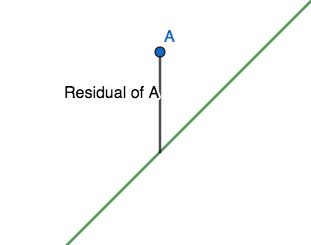
\includegraphics[scale=0.5]{images/residual}
  \item Let \(y = f(x) = mx+b\) be our line and let \(d(m,b)\) be the
    sum of the squares of the \(n\) residuals between our line and our data
    points. Write a formula for \(d(m,b)\) in sigma notation.
    \vspace{1in}
  \item In order to find our line of best fit, we must minimize
    \(d(m,b)\). Compute the first-order partial derivatives of \(d\)
    and set them 
    equal to zero.
    \vspace{2in}
  \item Now, we need to show that our critical point \((m,b)\) is a relative
    minimum. Compute the second partial derivatives \(d_{mm}, d_{mb},\) and
    \(d_{bb}\) and apply the second derivative test. To show \(D(m,b)
    >0\), you can use the
    famous \emph{Cauchy inequality} \[
      \left( \sum_{i=1}^n a_i^2 \right) \left( \sum_{i=1}^n b_i^2 \right) \geq
      \left( \sum_{i=1}^n a_i b_i \right) \text{ for all } a_i \geq 0, b_i
      \geq 0
    \]
  \end{enumerate}
\end{ex}
%%%%%%%%%%%%%%%%%%%%%%%%%%%%%%%%%%%%%%%%%%%%%%%%%% 
\end{document}
